\documentclass[letterpaper]{article}
\usepackage{tikz}
% Set tiny margins so it fits on one sheet
\usepackage[top=10mm,left=5mm]{geometry}
\usetikzlibrary{calendar}
% Get rid of blank page 1
\usepackage{atbegshi}
\AtBeginDocument{\AtBeginShipoutNext{\AtBeginShipoutDiscard}}

\begin{document}
% No page numbers
\pagestyle{empty}
\noindent
	
% Calendar on left
\begin{minipage}{.5\textwidth}
	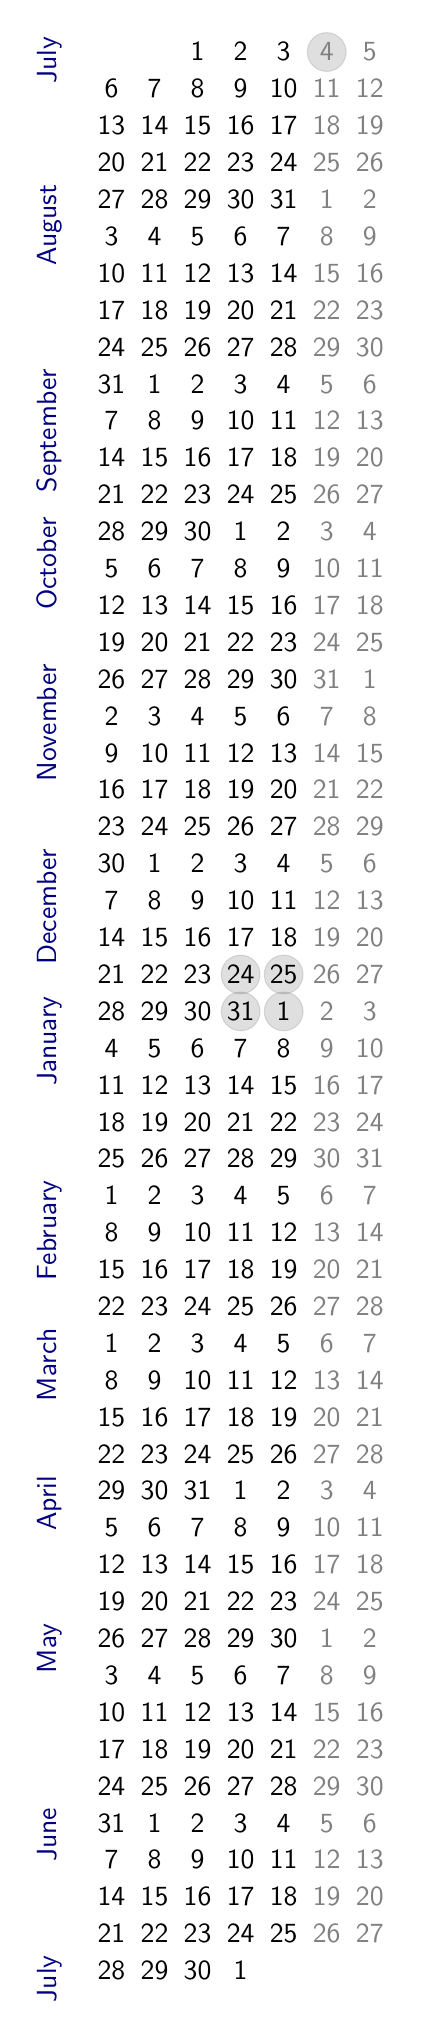
\begin{tikzpicture}
		normalsize\sffamily
		% Create a running 12 month calendar starting from the current month
		\calendar[dates=\year-\month-01 to \year-\month-01+365,week list,
		month label left vertical,month yshift=0pt,month text=\textcolor{blue!50!black}{\%mt},
		every day/.style={anchor=mid}]
		% Weekends are gray
		if (weekend) [gray]
		% Holidays are are highlighted with a gray circle
		if (
		equals=01-01,
		equals=07-04,  
		equals=12-24,
		equals=12-25,
		equals=12-31,
		equals=2024-03-29,
		equals=2024-03-31,
		equals=2024-05-27,
		equals=2024-06-19,
		equals=2024-09-02,
		equals=2024-11-28,
		equals=2025-01-20,
		equals=2025-04-18,
		equals=2025-04-20,
		equals=2025-05-26,
		equals=2025-06-19,
		equals=2025-09-01,
		equals=2025-11-27
		) {\draw[gray, fill=gray, fill opacity=0.25, draw opacity=0.25] (0,0.1em) circle (7pt);};
	\end{tikzpicture}
\end{minipage}
% Optional text on right
\begin{minipage}{.5\textwidth}
\setlength{\parskip}{5ex}
\IfFileExists{events.tex}{
	Example Event 1

Example Event 2

}{}
\end{minipage}
	
\end{document}
